%!TEX root = ../dokumentation.tex

\chapter{Einführung in die digitale Bildverarbeitung}
Die digitale Bildverarbeitung ist ein wesentlicher Aspekt der Informatik, welcher sich stetig weiterentwickelt.
Sie ermöglicht visuelle Daten zu interpretieren und die wertvollen Informationen daraus zu extrahieren. 

Die Wurzeln der Bildverarbeitung reichen bis in die 1960er Jahre zurück, als Computer aufkamen, die leistungsstark genug waren, 
um die Rechenanforderungen von Bilddaten zu bewältigen. Ihre Ursprünge findet sie in der Raumfahrtindustrie, wo es zur Verbesserung der
Qualität von Mondbildern Verwendung fand.~\cite{Brian_2017_spacefoundation}

Das Potenzial der Bildverarbeitung wurde jedoch schnell erkannt und fand schnell auch in anderen Bereichen eine Anwendung.
Im digitalen Zeitalter spielt sie eine Rolle in Bereichen wie der medizinischen Bildgebung über autonome Fahrzeuge, Überwachung und vielen mehr.
Das Wesen der Bildverarbeitung liegt in der Übersetzung einer visuellen Eingabe in eine mathematische Darstellung, welche von Computern verstanden werden kann.
Durch diese Umwandlung können Computer sie analysieren und manipulieren.~\cite{Kernel_2023_wikipedia}
Die folgenden Kapitel beschäftigen sich mit den Feinheiten der Bildverarbeitung.  

\section{Bildgrundlagen}

\subsection{Verständnis von Pixeln}
Pixel beschreiben die kleinste Einheit eines digitalen Bildes und sind somit essenziell für das Verständnis der Bildverarbeitung.
Jeder dieser Pixel beschreibt dabei einen einzelnen Punkt im Bild und hat einen bestimmten Pixelwert, welcher die Helligkeit oder Farbe 
widerspiegelt. In farbigen Bildern werden diese Pixel durch Tripletts von Farbwerten repräsentiert. Oftmals wird hierbei der RGB-Farbraum 
verwendet. RGB steht hierbei für die drei Farben des Tripletts: Rot, Grün, Blau.~\cite{J.F._Blinn_2005_ieee}

\subsection{Bildrepräsentation}
Ein digitales Bild lässt sich als zweidimensionale Funktion \(f(x,y)\) darstellen, bei der \(x\) und \(y\) die räumliche Koordinaten sind
und die Amplitude von \(f\) zu jedem Paar \((x,y)\) die Intensität oder den Grauwert des Bildes an dem Punkt repräsentieren.
Bei farbigen Bildern besteht jedes Pixel aus einer Kombination von Primärfarben. In den meisten Fällen werden diese als RGB dargestellt. 
Die Digitalisierung von Bildern ermöglicht die Anwendung verschiedener Operationen, um es zu manipulieren oder zu analysieren. 

\subsection{Farbräume}
Farbräume sind mathematische Modelle zur Darstellung von Farben. Ihr Ziel ist es Farben so zu beschreiben, dass sie für das menschliche Auge
sinnvoll sind.

\subsubsection{RGB-Farbraum}
Der am weitesten verbreitete Farbraum ist der RGB-Farbraum. Hierbei werden die Primärfarben Rot, Grün und Blau in verschiedenen
Intensitäten gemischt, um möglichst viele Farben darzustellen. Jede Farbe wird somit durch ein Triplett von Werten dargestellt.
Jeder dieser Werte beschreibt dabei die Intensität der jeweiligen Primärfarbe. Beispielsweise entspricht ein Triplett
\((0,0,0)\) Schwarz, da keine Farbe vorhanden ist, während \((255,0,0)\) Rot entspricht.
Im digitalen Kontext ist der RGB-Farbraum besonders dominant, da er für die Farbdarstellung auf Bildschirmen zuständig ist.
Die einzelnen Pixel auf dem Bildschirm emittieren Licht in den Grundfarben und der Nutzer nimmt den Pixel als die additive Mischung dieser 
Farben auf.~\cite{Vladimir_Chernov_2023_sciencedirect}

\subsubsection{HSV-Farbraum}
Ein weiterer verbreiteter Farbraum ist HSV (Hue, Saturation, Value), welcher oftmals intuitiver als der 
RGB-Farbraum ist.
\begin{figure}[ht]
    \centering
    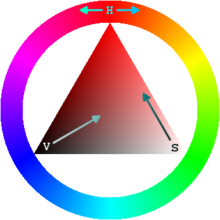
\includegraphics[scale=0.6]{images/HSV.png}
    \caption{HSV Farbraum Palette}
\end{figure}
\begin{itemize}
    \item Hue (Farbton): Der Farbton wird auf einer kreisförmigen Skala dargestellt. 
    0 oder 360 entspricht Rot, 120 Grün und 240 Blau. Die Zwischenwerte sind Mischungen der Farben.
    \item Saturation (Sättigung): Die Sättigung gibt die Intensität der Farbe an. 
    Eine Sättigung von 0 entspricht weiß, während eine Sättigung von 100 eine reine Farbe darstellt.
    Somit erscheinen Farben mit geringen Sättigungen als blass und Farben mit hoher Sättigung als voll.
    \item Value (Helligkeit): Dieser Wert spiegelt die Helligkeit oder Intensität des Lichts wider, welches von der Farbe ausgeht.
    Ein Wert von 0 stellt also Schwarz dar, während ein Wert von 100 eine Farbe in voller Helligkeit darstellt.
\end{itemize}
Der HSV-Farbraum findet vor allem Anwendung in Aufgaben, bei denen eine intuitive Steuerung wichtig ist. Beispielsweise das Ausfiltern einer Farbe durch den Nutzer.~\cite{Vladimir_Chernov_2023_sciencedirect}
\subsubsection{Graustufen}
Grayscale, oder Graustufen bezeichnen eine Darstellung von Bildern, bei welcher der Wert jedes Pixels die Intensität der Information wiedergibt.
In einem Graustufenbild kann jeder Pixel als ein unterschiedlicher Grauton angesehen werden, der von Schwarz (minimale Intensität) 
bis Weiß (maximale Intensität) reicht. Die verschiedenen Töne zwischen diesen Extremen entsprechen dann den Intensitätstufen des Lichts.
Graustufenbilder werden oft bei Aufgaben verwendet, bei denen die Farbinformationen nicht notwendig sind und ablenken können. 
Beispielsweise werden Graustufenbilder verwendet, wenn der Computer eine bestimmte Form in einem Bild finden soll, da 
Bildverarbeitungstechniken wie die Kanten-Erkennung mit Intensitätsinformationen arbeiten.
Die Verwendung von Graustufen kann außerdem die Rechenkomplexität verringern und somit die Leistung verbessern.

Im Kontext der Farbraum Umwandlung kann ein RGB-Bild oft in Graustufen umgewandelt werden, indem ein gewichtetes Mittel der RGB-Werte genommen wird. 
Diese Gewichte berücksichtigen die menschliche Wahrnehmung, da das menschliche Auge empfindlicher auf Grün und weniger empfindlich auf Blau reagiert.
Die typische Formel zur Umwandlung von RGB in grayscale ist \(grayscale = 0,299*R + 0,587*G + 0,114*B\).~\cite{Dr._Daniel_Slieter_2023_dhbw-stuttgart}

\section{Bildvorverarbeitung}
Die Bildvorverarbeitung stellt eine kritische Stufe in der Bildverarbeitung dar. Ihre Hauptaufgabe besteht darin, 
die Qualität und Lesbarkeit eines Bildes zu verbessern und das Fehlerpotenzial für nachfolgende Dateninterpretationen zu reduzieren.

\subsection{Rauschunterdrückung}
Rauschen ist in der Physik allgegenwärtig und bezeichnet eine Übertragung eines Signals mit einem ungewollten Störsignal.
Meistens handelt es sich beim Rauschen um einen stochastischen Prozess, was dazu führt, dass die verschiedenen Arten des Rauschens sich mit
ihren jeweiligen Wahrscheinlichkeitsverteilungen modellieren lassen.
Das Rauschen kann verschiedene Formen annehmen, wie zum Beispiel das additive / multiplikative Gauß'sches Rauschen, ungleich verteiltes Rauschen
und Salt-and-Pepper-Rauschen. 

\begin{figure}[ht]
    \centering
    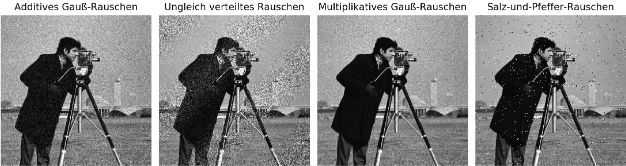
\includegraphics[scale=0.8]{images/noise.png}
    \caption{Verschiedene Arten des Rauschens}
\end{figure}

Rauschunterdrückungsalgorithmen zielen darauf ab, die Auswirkungen dieser Verzerrungen zu minimieren und die Bildqualität zu verbessern.
Je nach Art des Rauschens werden verschiedene Algorithmen benutzt.~\cite{Hannes_Bonasch_2023}

\subsection{Bildverbesserung}
Bildverbesserungstechniken werden verwendet, um visuell aufschlussreichere Bilder zu generieren, 
sowie eine Vereinfachung der nachfolgenden Signalverarbeitung und der automatischen Bildauswertung zu schaffen. Ein Beispiel für die 
Bildverbesserung ist die Bildverschärfung. Details von Bildern hängen mit einer höheren räumlichen Frequenz zusammen. Wenn diese Frequenz 
verstärkt wird, erscheint das Bild scharfer. Jedoch kann die Verschärfung auch zu weiteren Störungen führen und es muss darauf geachtet werden,
dass der durchschnittliche Bildwert konstant bleibt.~\cite{Jürgen_Beyerer_Fernando_Puente_León_Christian_Frese__2023_springer}

\subsection{Farbraum Umwandlung}
Da verschiedene Farbräume verschiedene Informationen über ein Bild liefern, kann die Umwandlung eines Bildes von einem Farbraum in einen anderen 
vorteilhaft sein. Beispielsweise wird der RGB-Farbraum oft für die Bilddarstellung verwendet während der HSV-Farbraum für die farbbasierte Bildsegmentierung
effektiver ist. Ebenso kann die Umwandlung in ein grayscale Bild die Daten vereinfachen und ist somit vorteilhaft für Aufgaben, bei denen die Farbinformationen
unnötig sind.~\cite{Noor_A._Ibraheem_2012_psu}

\section{Farbfilterung}
Die Farbfilterung gehört zu den wichtigsten Komponenten der digitalen Bildverarbeitung. Sie ist entscheidend für eine Vielzahl von Anwendungen,
wie der Objekterkennung, Gesichtserkennung und Merkmalsextraktion.

Die Farbfilterung beschäftigt sich in erster Linie mit der Trennung oder Hervorhebung bestimmter Farbbereiche in einem Bild. Dieser Prozess wird hauptsächlich durch
die Definition eines bestimmten Farbbereichs oder mehrerer Farbbereiche im Farbraum eines Bildes erleichtert. Anschließend werden Pixel, die innerhalb 
dieser festgelegten Bereiche fallen, beibehalten, während die anderen in der Regel auf Schwarz gesetzt werden, 
wodurch die gewünschten Farbkomponenten effektiv isoliert werden. Es gibt verschiedene Farbfilterungen, je nach Farbbereich. 
Die populärsten sind jedoch HSV-Farbfilterung und Graufilterung. Der Grund für die Nutzung des HSV-Filters statt eines RGB-Filters 
ist die Entkopplung der Farb- und Helligkeitsinformationen. Der Filter wird in Aufgaben verwendet, bei denen die Robustheit gegenüber 
Beleuchtungsänderungen relevant ist. 

\section{Formerkennung}
Neben der Farbfilterung ist die Formerkennung eine grundlegende Rolle in der Bildverarbeitung und unverzichtbar in einer Vielzahl von Anwendungen,
die von Objekterkennung und Objektverfolgung über medizinische Bildgebung bis hin zur maschinellen Bildverarbeitung reichen. Im Folgenden wird 
die Mechanik der Formerkennung erläutert und verwendete Methoden aufgezeigt.

\subsection{Kanten-Erkennungsmethoden}
Die Kanten-Erkennung ist einer der Schlüsselschritte in der Formerkennung. In erster Linie befasst sie sich mit der Identifizierung von Punkten in einem Bild,
an denen die Helligkeit stark wechselt, beziehungsweise Punkte an denen der Gradient der  Bildintensitätsfunktion hoch ist. Für diesen Zweck wurden diverse
Methoden entwickelt. Die bekanntesten sind die Sobel- und Canny-Operatoren. Die Operatoren unterscheiden sich dabei in ihren Ansätzen und 
liefern unterschiedliche Ergebnisse, abhängig von den spezifischen Anforderungen der Anwendung.~\cite{AHMED_SHIHAB_AHMED_2018_jatit}

\subsubsection{Sobel-Operator}
Der Sobel-Operator wird verwendet,  um die Gradienten der Bildintensität an jedem Pixel zu bestimmen und 
um Regionen zu markieren, falls deutliche Intensitätskontraste auftreten. Er läuft durch das Bild mit einem Paar von 3$\times$3-Kerneln, 
die auf senkrecht und waagrecht zur Pixelmatrix verlaufende Kanten reagieren. Beispielhafte Kernel könnten wie folgt aussehen:

\begin{figure}[h!]
\centering
\begin{align*}
    A &= \begin{bmatrix}
        -1 & 0 & 1 \\
        -2 & 0 & 2 \\
        -1 & 0 & 1
    \end{bmatrix},
    & B &= \begin{bmatrix}
        -1 & -2 & -1 \\
        0 & 0 & 0 \\
        1 & 2 & 1
    \end{bmatrix}
\end{align*}
\caption{(A) Sobel vertikal-Operator (B) Sobel horizontal-Operator}
\end{figure}

Die resultierenden Kanten werden als Grauwertbilder dargestellt, 
bei denen Kanten auf einem schwarzen Hintergrund zu sehen sind. Die Ausgabe kann anschließend binarisiert werden, 
um Kanten klar vom Rest des Bildes zu trennen und für weitere Bildverarbeitungsaufgaben verwendet werden.~\cite{AHMED_SHIHAB_AHMED_2018_jatit}

\subsubsection{Canny-Operator}
Im Gegensatz dazu verwendet der Canny-Operator eine Reihe von Schritten, um präzisere und weniger störanfällige Kanteninformationen zu erzeugen.
Er beginnt mit der Glättung des Bildes durch eine Gaußsche Glättung, um das Rauschen zu reduzieren. Anschließend wird ein Schritt durchgeführt, 
welcher dem Sobel-Operator ähnelt, um die Gradientenmagnituden und -richtungen zu bestimmen. Die Kanten werden nun durch eine Nicht-Maximum-Unterdrückung
geschärft. Im letzten Schritt wird die Schwellenwertbildung mit Hysterese angewendet, um sicherzustellen, dass nur die stärksten Kanten im Resultat 
zu sehen sind.

Die Wahl zwischen den Operatoren hängt stark vom Anwendungsfall ab. Die Implementation des Sobel-Operators ist einfacher, jedoch ist er anfälliger 
für Bildrauschen und kann bei feinen Kanten ungenau sein. Der Canny-Operator ist dem Sobel-Operator damit in der Qualität der Ergebnisse überlegen,
jedoch steigt durch die erhöhte Komplexität auch die Anforderungen an die Rechenleistung und den benötigten Speicher.~\cite{AHMED_SHIHAB_AHMED_2018_jatit}

\subsection{Konturerkennung}
Konturen sind ein weiteres wichtiges Merkmal in der Bildverarbeitung, um einen Rückschluss auf Objekte zu geben. Die Erkennung beinhaltet das 
Gruppieren von Kantenpixeln zu zusammenhängenden Kurven. Konturerkennungstechniken bieten somit eine Möglichkeit zur Erkennung und Visualisierung
von Objektgrenzen und liefern eine ganzheitliche Darstellung der Form im Vergleich zu den isolierten Kantenpixeln.~\cite{Xin-Yi_Gong_2018_springer}

\subsection{Formerkennung}
Nach der Erkennung von Kanten und Konturen besteht der nächste Schritt in der Erkennung von Formen. Das geschieht durch den
Vergleich der erkannten Form mit einem Satz bekannter Formen. Dieser Prozess kann einfache geometrische Formen (Kreise, Quadrate, etc.) 
oder komplexere Formen beinhalten, sofern diese erlernt wurden. Die Formerkennung geht oft Hand in Hand mit einem Ansatz des maschinellen Lernens
und Mustererkennungsalgorithmen, um die Formen zu klassifizieren.~\cite{Sambarta_Dasgupta_2009_springer}

\section{Bildsegmentierung}
Die Bildsegmentierung ist entscheidend für die Extraktion spezifischer Merkmale oder Objekte in einem Bild. Im Wesentlichen transformiert sie ein
Bild in eine Ansammlung von Regionen mit identifizierbaren Eigenschaften. Diese Transformation liefert eine Darstellung des Bildes, die topologische
und geometrische Informationen liefert und als Grundlage für die weitere Bildanalyse und Interpretation dient.

\subsection{Techniken zur Bildsegmentierung}
Je nach Anwendungsfall gibt es verschiedene Techniken zur Bildsegmentierung.

\subsubsection{Schwellenwertsetzung}
Die Schwellenwertsetzung ist wegen ihrer Einfachheit weit verbreitet. Ihr Ziel ist es, den Vordergrund eines Bildes vom Hintergrund zu trennen, 
indem ein Graustufen- oder Farbbild in ein Binärbild umgewandelt wird.

\begin{figure}[h]
    \centering
    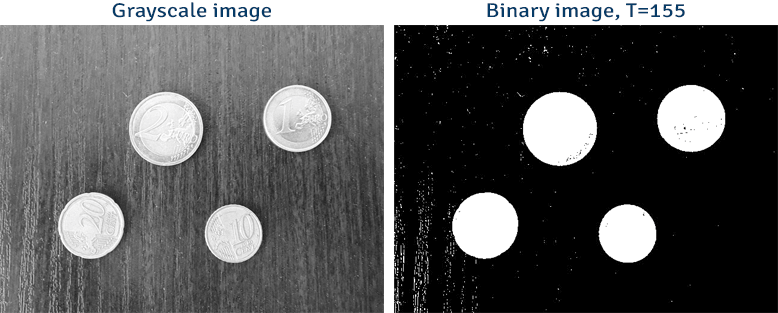
\includegraphics[scale=0.5]{images/threshholding.png}
    \caption{Schwellenwertsetzung Beispiel}
\end{figure}

Wie in Abbildung 3.4 zu sehen ist, wird ein zunächst ein Schwellwert gewählt. Je kleiner dieser ist, desto kleinere Objekte werden erkannt.
Anschließend werden alle Pixelintensitätswerte über oder unter diesem Schwellwert auf einen bestimmten Wert gesetzt, um die gewünschte Segmentierung
zu erreichen. Ein Vorteil der Schwellenwertsetzung ist die einfache Implementation, jedoch kann es bei variablen Lichtverhältnissen zu fehlerhaften
Ergebnissen kommen. 

\subsubsection{Clustering}
Eine andere Gruppe von Techniken zur Bildsegmentierung umfasst das Clustering. Ein Beispiel für diese Technik ist K-means, 
welcher die Pixel mit ähnlichen Attributen zusammenfasst. Der K-means-Algorithmus segmentiert dabei ein Bild in K Cluster, 
wobei jedem Pixel das Cluster mit dem nächstgelegenen mittleren Intensitätswert oder Farbvektor zugeordnet wird. 
Trotz der Vielseitigkeit dieses Algorithmus, reagieren die Ergebnisse sehr empfindlich auf die Parameter Auswahl und der Algorithmus ist
sehr rechenintensiv.~\cite{G.B._Coleman_1979_ieee}

\section{Bildtransformation}
Bildtransformationen sind Operationen in der Bildverarbeitung, die Bilder zur Analyse, Interpretation oder Visualisierung modifizieren. 
Diese Operationen lassen sich in räumliche Transformationen, die die räumlichen Attribute des Bildes verändern, 
und Frequenzbereich-Transformationen, die den Frequenzinhalt des Bildes manipulieren, unterteilen.

\subsection{Räumliche Transformationen}
Räumliche Transformationen sind Bildoperationen, die die Position und Ausrichtung der Pixel in einem Bild ändern 
und dabei ihre Nachbarschaftsbeziehungen beibehalten.

\subsubsection{Skalierung}
Die Skalierung ist eine Transformation, die die Größe eines Bildes ändert. Sie kann sowohl eine Vergrößerung als auch eine Verkleinerung sein, 
beide verändern die Breite und Höhe des Bildes. Dabei ist es entscheidend, das Seitenverhältnis während der Skalierung beizubehalten, 
um eine Verzerrung des Bildes zu verhindern.

\subsubsection{Rotation}
Die Rotation ist eine Transformation, die die Ausrichtung eines Bildes ändert. 
Sie beinhaltet das Drehen der Pixel des Bildes um einen bestimmten Punkt, typischerweise das Bildzentrum, um einen bestimmten Winkel. 
Wie andere räumliche Transformationen muss darauf geachtet werden, Pixelinterpolation zu vermeiden und die Bildqualität zu erhalten.
Die Pixelinterpolation beschreibt dabei das Problem, dass die ursprünglichen Pixel nicht in das Pixelgitter des neuen Bildes passen.
Dann muss eine Entscheidung getroffen werden, welcher Wert dem neuen Pixel zugeordnet wird.~\cite{Don_Lancaster_2007_ollintec}

\subsubsection{Translation}
Die Translation ist eine räumliche Transformation, die ein Bild in x- und/oder y-Richtung verschiebt. 
Dabei wird jeder Pixel an einen neuen Ort verschoben, ohne seinen Wert zu ändern.

\subsection{Transformationen im Frequenzbereich}
Transformationen im Frequenzbereich beinhalten die Umwandlung eines Bildes vom Raum- in den Frequenzbereich, 
bei dem die Informationen des Bildes in Bezug auf ihren Frequenzinhalt dargestellt werden.
Der Frequenzinhalt eines Bildes bezieht sich auf die Rate, mit der die Pixelintensitäten (oder Farben) im Bild ändern. 
Diese Änderungsrate wird in Form von Frequenzen gemessen.

\subsubsection{Fourier-Transformation}
Die Fourier-Transformation ist ein Standardwerkzeug zur Analyse des Frequenzinhalts eines Bildes. 
Sie zerlegt ein Bild in seine Sinus- und Kosinus-Komponenten und zeigt die periodischen Strukturen des Bildes und ihre Ausrichtungen auf. 
Die resultierende Darstellung ist komplex und enthält sowohl Amplituden- als auch Phaseninformationen, die beide notwendig sind, 
um das Originalbild vollständig zu rekonstruieren.~\cite{S._Sridhar_2014_mecs-press}

\subsubsection{Wavelet-Transformation}
Eine weitere Technik zur Frequenzbereichsanalyse ist die Wavelet-Transformation. Im Gegensatz zur Fourier-Transformation, 
welche das Bild global betrachtet, verwendet die Wavelet-Transformation Wavelets, um das Bild lokal zu analysieren 
und eine Zeit-Frequenz-Darstellung zu liefern. Diese Eigenschaft ist nützlich für die Analyse von Bildern mit 
nicht-stationären Signalen oder mit Strukturen auf mehreren Skalen.~\cite{S._Sridhar_2014_mecs-press}

\subsection{Anwendungen von Bildtransformationen}
Bildtransformationen spielen eine entscheidende Rolle in verschiedenen Anwendungen. Räumliche Transformationen werden in der Bildregistrierung verwendet, 
bei der Bilder zum Vergleich ausgerichtet werden, und in der Datenvergrößerung für maschinelles Lernen, bei der Bildvarianten erstellt werden, 
um Trainingsdaten zu erweitern. 
Transformationen im Frequenzbereich hingegen werden in der Bildfilterung, Kompression und Rauschreduzierung verwendet.
Zum Beispiel wird die Fourier-Transformation in der MRT-Bildgebung eingesetzt. Die Wavelet-Transformation wird in der JPEG2000-Kompression verwendet, welche 
einen verbesserten Nachfolger des JPEG-Standards darstellt.
Durch diese Anwendungen tragen Bildtransformationen erheblich zur Fähigkeit bei, visuelle Daten zu analysieren, zu interpretieren und zu nutzen.~\cite{H._Burkhardt_uni-freiburg}

\section{Merkmalsextraktion}
Die Merkmalsextraktion besteht darin, relevante Informationen aus einem Bild zu extrahieren. Dieser Prozess ermöglicht eine Reduzierung 
der Datenmenge bei gleichzeitiger Beibehaltung der wesentlichen Details, wodurch Aufgaben wie Bilderkennung, 
Objekterkennung oder das Training von maschinellem Lernen erleichtert werden.

Merkmale können als messbare Eigenschaften beobachteter Auffälligkeiten definiert werden. Im Fall von Bildern entsprechen diese Merkmale 
oft ausgeprägten Elementen der Bildstruktur, wie Kanten, Ecken oder Bereiche mit einer bestimmten Textur oder Farbe. 
Ziel der Merkmalsextraktion ist es, das Bild so zu repräsentieren, dass die Beschreibung vereinfacht oder das Potenzial 
für nachfolgende Analysen oder Klassifikationen verbessert wird.~\cite{Shambhavi_Jain_2017_ieee}

\subsection{Techniken zur Merkmalsextraktion}
Es gibt diverse Techniken, welche zur Extraktion von Merkmalen aus Bildern verwendet werden können. 
Zwei populäre Techniken, die häufig im Bereich der Bildverarbeitung und Computer Vision verwendet werden, 
sind das \ac{SIFT} und das \ac{SURF}.~\cite{Shambhavi_Jain_2017_ieee}

\subsubsection{SIFT}
\ac{SIFT} ist eine Methode zur Erkennung und Beschreibung lokaler Merkmale in Bildern. 
Die mit dieser Methode extrahierten Merkmale sind immun gegenüber Bildskalierungen und -rotationen 
und zeigen eine robuste Übereinstimmung über einen erheblichen Bereich von Verzerrungen, Änderungen des 3D-Blickpunkts, 
Hinzufügen von Rauschen und Änderungen der Beleuchtung.~\cite{Shambhavi_Jain_2017_ieee}

\subsubsection{SURF}
\ac{SURF} ist ein weiterer Bild-Deskriptor. Es ähnelt \ac{SIFT} in vielen Aspekten, ist aber schneller und robuster gegenüber Bildtransformationen, 
was es für Echtzeitanwendungen geeignet macht und perfekt für Aufgaben ist, die eine schnelle Merkmalsextraktion erfordern.~\cite{Shambhavi_Jain_2017_ieee}